\chapter{FPGA tervezés}
\label{sec:fpga-desing-begining}

A Nintendo Entertainment System hardveres komponenseinek újratervezése során az ISE Design Suit szoftvert és hardver leíró nyelvnek pedig a Verilog-ot választottam. A tervezés fő szempontja a beláthatóság, céltudatosság és tesztelhetőség volt, ez elengedhetetlen egy nagyobb projekt fejlesztése során. A megtervezett chipeknek az összehangolt és hibátlan (az eredeti NES hardverrel megegyező) működését követően léptem tovább a következő fejlesztési egységre.

A következőkben a diplomatervezés során tervezett és tesztelt hardveres komponensek működését és felépítést fogom bemutatni, az úgynevezett "top-down" elv alapján. Ennek jelentése, hogy először a teljes rendszer kapcsolatát mutatom be, majd ezt követően térek ki a különböző elemek részletes működésére.

\begin{figure}[H]
	\centering
	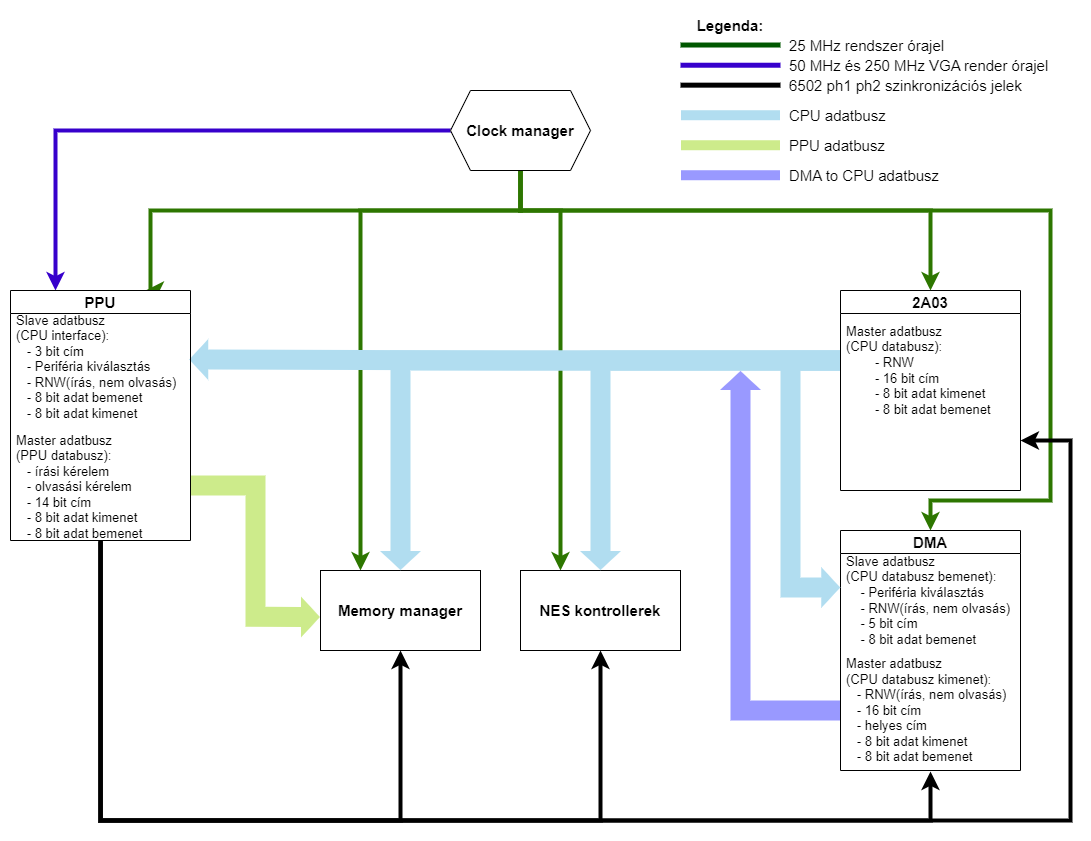
\includegraphics[width=150mm, keepaspectratio]{figures/FPGA-toplevel-diagram}
	\caption{Megvalósult FPGA projekt (nes\_top) működési diagramja} 
	\label{fig:FPGA-toplevel-diagram}
\end{figure}
%\section{Rendszer blokkvázlat bemutatása}

Az FPGA tervezés során a különböző funkciókat ellátó hardveres elemek (a NES különböző chipjeinek) leírását modulokra osztottam. Ezeket a modulokat és a köztük lévő logikai kapcsolatot láthatjuk \aref{fig:FPGA-toplevel-diagram} ábrán.

Az ábrán a modulok közti két fő adatkapcsolatot láthatjuk az első a vastagabb nyilak, amelyek több vezetéket foglalnak magukba (ezek a nyilak kezdőpontján fel vannak tüntetve). A második pedig a rendszer órajelek. Ide tartozik a rendszer órajelből elő állított, $phi_1$ és $phi_2$ szinkronizációs jelek is.



\section{Adatbuszok implementálása}

A NES eredeti belső adatbuszkapcsolatait alapul véve, két fő adatbuszt különböztetünk meg a CPU és a PPU adatbuszt. 

A PPU adatbusz struktúrájában egyszerűbb csupán a memória menedzser modullal kommunikál. A modulban található név tábla (NT) memóriát írja és olvassa, illetve a karakter ROM tartalmát olvassa. 

A CPU adatbusz működése a DMA miatt egy fokkal bonyolultabb. Alap esetben a CPU az adatbuszán keresztül éri el a címtartományában található különböző perifériák regisztereit/memóriáit. A slave interfészek implementálása során ügyeltem arra hogy a különböző hardveres komponensek minél egyszerűbb interfésszel fogadják a CPU adatbuszát (ezzel egyszerűsítve a szintetizálandó hardveren), ez \aref{code:cpu-databus-simplification} hardverleírásban is látható. A DMA működése során viszont a helyes cím kiadásával a periféria átveszi a processzor adatbuszát, ilyen kor ő végez hozzáféréseket a perifériákhoz. A helyes cím kiadása mellett a DMA elveszi a processzor Ready jelét is ezzel blokkolva cpu működést és megakadályozva a busz több periféria általi meghajtását. A különböző modulok kimeneti jelei úgy lettek megtervezve, hogy csak megfelelő időzítés mellet adjanak ki adatokat így \aref{code:cpu-data-bus} hardverleírásban is látható módon a különböző kimenetek egyszerű vagy kapcsolatával tudjuk adatbuszunkat összegezni.

\begin{lstlisting}[caption={CPU adatbuszt befolyásoló DMA jelek}, label={code:cpu-data-bus}, style=prettyverilog]
// CPU data in
wire [7:0] cpu_din = (memory_manager_cpu_din | ppu_to_cpu_din | controller_cpu_din);

// DMA and CPU outputs
assign cpu_addr = (dma_cpu_avalid) ? (dma_cpu_addr) : (nes6502_addr);
assign cpu_dout = (dma_cpu_dout | nes6502_dout);
assign rnw = ~(~dma_cpu_rnw | ~nes6502_rnw);\end{lstlisting}

A különböző interfészek egyszerűsítése során \aref{tab:CPU-Memory} táblázatban és \aref{sec:NT-AT-mirroring} fejezetben bemutatott tükrözés "mirroring" jelenségét használtam ki. Ennek alapja hogy csupán a címregiszter adott bitjeit figyeljük, például PPU regiszterek esetén az alsó három bitet. Ezzel párhozamosan pedig megpróbálunk egy megfelelő kiválasztó jelet generálni a chiphez, PPU esetén a felső három bit fixálja a \$2000 - \$3FFF-ig tartó cím tartományt. Ilyen egyszerűsítést alkalmaztam a kontrollerek és DMA interfész esetén is (\ref{code:cpu-databus-simplification}).

\begin{lstlisting}[caption={A CPU adatbusz interfészek egyzserüsítése}, label={code:cpu-databus-simplification}, style=prettyverilog]
// PPU Slave interface bemenet
.slv_mem_addr(cpu_addr[2:0]),      				// register interface reg select (#2000-#2007)
.slv_mem_cs((cpu_addr[15:13] == 3'b001)), 		// register interface enable (#2000 - #3FFF just when it is active)

// Controller inputs
.cpu_data_in(cpu_dout[0]), //just one bit the $4016 write strobe

// DMA Slave databus
.slv_mem_select((ag6502_addr[15:14] == 2'b01)),  
.slv_mem_addr(ag6502_addr[4:0]),\end{lstlisting}

\section{Működési órajel választása}

Egyik első feladat FPGA tervezés során a hardver átgondolását követően, a rendszerórajel kiválasztása. Erről a fő órajelről fogjuk működtetni a szinkron tárolóinkat, memória elérésünket és az összes perifériánk időzítésének ez lesz az alapja. Hardverünkben használhatunk több kiemelt órajelet is ahol magasabb órajelre van szükségünk, ilyen például a HDMI jel előállításához szükséges bit órajel. A működési órajeleinknek a többi FPGA-n található jeltől elkülönített helyen a globális órajel osztó hálózatban folynak, ez biztosítja rendszerünk számára, hogy minden SLICE-hoz ugyanakkor érjen el az órajelünk. Erre az órajelosztó hálózatra csat lakozik a külső órajel forrásunk is. Illetve a PLL és DCM hardveres elemek amelyek lehetővé teszik az órajelek frekvenciájának változtatását.

A NES kártyán egy 50 MHz-es külső órajel forrást helyeztem el.  \aref{sec:picture-creation-ideas} fejezet alapján a rendszer órajelemet a megjelenítésnek kell alárendelnem. Tehát a működési órajelemet és egyben a pixel órajelemet is 25 MHz-nek választom. A beérkező 50MHz-ből a PLL helyes beállítása során elő állítottam 25 MHz-et és 250 MHz-et. A VGA kép generálásához szükségem lesz mind a három órajelre, a 25 Mhz a pixel órajelem (erre a jelre kell előállítanom a  24 bites RGB értékeimet), az 50 MHz az 5 bites párhuzamos-soros átalakítókhoz kellenek (stobe jelek) végül pedig a 250 MHz-el fogom kiadni a biteket a HDMI differenciális adatvezetékei számára. 

\begin{lstlisting}[caption={6502 $phi_1$ és $phi_2$ vezérlő jelek előállítása}, label={code:6502-clocksignals}, style=prettyverilog]
reg  clkgen_cnt_en_clr;
wire clkgen_cnt_en_set = (x_rendercntr == (ODDFRAME_END_OF_BG_RENDERING_LINE + 4));
always @(*) 
begin
	if (background_enabled && oddframe && (y_renderingcntr == PRERENDERING_ROW))
		clkgen_cnt_en_clr <= (x_rendercntr == ODDFRAME_END_OF_BG_RENDERING_LINE);
	else
		clkgen_cnt_en_clr <= 1'b0;	
end

// clock genereation enable
reg		clkgen_cnt_en;
always @ (posedge clk)
begin
	if (rst || (x_rendercntr == END_OF_BG_RENDERING_LINE) || clkgen_cnt_en_clr)
		clkgen_cnt_en <= 1'b0;
	else
		if ((x_rendercntr == FIRST_SCANLINE_PIXEL) || clkgen_cnt_en_set)
			clkgen_cnt_en <= 1'b1;
end	

//clock generation timer
reg	[3:0]	clkgen_cnt;
always @ (posedge clk)
begin
	if (rst)
		clkgen_cnt <= 4'd0;
	else
		if (clkgen_cnt_en)
			if (clkgen_cnt == 4'd11)
				clkgen_cnt <= 4'd0;
			else
				clkgen_cnt <= clkgen_cnt + 4'd1;
end

always @ (posedge clk)
begin
	ph1_rising	<= clkgen_cnt_en & (clkgen_cnt == 4'd0);
	ph1_falling <= clkgen_cnt_en & (clkgen_cnt == 4'd5);
	ph2_rising	<= clkgen_cnt_en & (clkgen_cnt == 4'd6);
	ph2_falling <= clkgen_cnt_en & (clkgen_cnt == 4'd11);
end\end{lstlisting}

Ezekből az órajelekből kell előállítani a NES hardver számára a megfelelő kiválasztó jeleket. Az NTSC NES-ben található MOS 6502 1.789773 MHz-es bemeneti $phi_0$ órajellel rendelkezik. Ebből hozza létre a fázis tolt $phi_1$ és $phi_2$ időzítési órajelet. A $phi_2$ órajel lefutó élére történik a periféria adtok olvasása. 

A projekt VGA rendrelését úgy implementáltam, hogy amíg a PPU képgenerálást kiegészíti a hardver VGA jellé, addig a PPU és vele együtt az egész NES hardver egy alvó állapotban várakozik. Ezt a $phi_1$ és $phi_2$ jelek megfelelő időben történő generálásával és késleltetésével tudtam kialakítani. Ezt láthatjuk \aref{code:6502-clocksignals} hardverleírásban. A Verilog kód első felében azt láthatjuk, hogy a PPU aktív kép generálása során az óra jel generálásáért felelős számláló engedélyezve van, viszont a képalkotás végeztével (VGA blanking terület) a számlálót tiltjuk. Legfelül pedig az látható, hogy az eredeti PPU megkülönböztette minden második kép generálását (páratlan) úgy, hogy specifikus pixeleket kihagyott a generálásból (clkgen\_cnt\_en\_clr jel). Ezt követően pedig kiszámolható, hogy a 25 MHz-es órajelünkre működtetett számlálót, ha 11-re nullába állítjuk, akkor az első hat óra jel alatt aktív a $phi_1$ és a második alatt a $phi_2$. Ha ehhez még hozzá számoljuk a számláló megfelelő engedélyezését, ~1.8 Mhz körüli értéket kapunk. Ezen órajelek éldetektálása fogja adni a NES hardver engedélyező jeleit \ref{fig:FPGA-phi1-phi2}.

\begin{figure}[H]
	\centering
	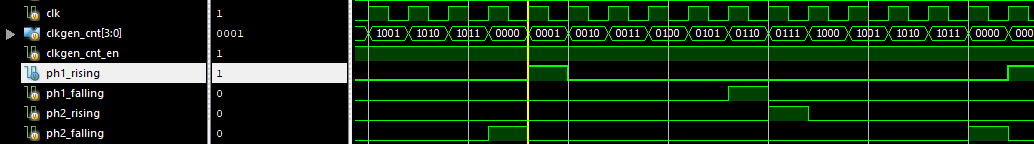
\includegraphics[width=150mm, keepaspectratio]{figures/fpga-ph1-ph2}
	\caption{MOS 6502 órajel generálása (FPGA sim)} 
	\label{fig:FPGA-phi1-phi2}
\end{figure} 

\section{Picture Process Unit}
\label{sec:PPU-FPGA}

A PPU időzítésének és működésének alap pillérét két számláló, egy horizontális és vertikális képzi. Ezek végig követik a teljes eredeti képgenerálását és ezzel együtt a új HDMI-n keresztül történő képgenerálást is szinkronban. A \ref{sec:picture-creation-ideas} fejezetben bemutatott két módszer közül az egyszerűbb megoldást választottam a képgenerálás megalkotására. Tehát minden egyes NES pixelt felnagyítok 2 x 2 pixellé ezzel egy pixelesebb, de élesebb képet kapva végeredményként (amely jobban hasonlít az eredeti konzol képére).

Az NTSC PPU képalkotását \aref{sec:NTSC-PPU-frame} függelékben láthatjuk. Az eredeti hardver, a 0-239-ig tartó sorokban, az 1. pixeltől kedve a 256. pixelig minden egyes órajelben elő állít egy pixelt a kompozit jelbe. Ha ezt a képalkotást szeretnénk szinkronba hozni a 640 x 480 pixeles vga jel elő állításával (az eredeti pixelek "nagyításával"), ami 800 pixelt jelent horizontálisan és 525 sort vertikálisan (blanking pixelekkel együtt). Akkor egy 1600-as horizontális számlálóval, és egy 261-ig tartó vertikális számlálóval megoldható, hogy egy PPU sor ideje alatt két sor VGA képet küldjünk ki. Természetesen így egy puffereléssel el kell csúsztatnunk a VGA képalkotást a PPU-hoz képest és az 1600-as PPU sort minden második rendszer órajelre kell mintavételeznünk. Ennek függvényében \aref{sec:NTSC-PPU-frame} függelékben látható állapotgépek állapotait is meg kell hosszabbítani, még hozzá úgy, hogy a képen látható horizontális pixel órajel, minden pixele az FPGA képalkotásban négy rendszer órajelnek feleljen meg. Erre a két számlálóra épül a teljes chip időzítése a PPU modulban. 

	\subsection{CPU által elérhető regiszterek és CPU adatbusz}
	\label{sec:CPU-databus-ppu_reg}
	
	Először is tekintsük meg a CPU adatbusz címének dekódolását és az ebből elő állított vezérlő jeleket a PPU számára \ref{code:CPU-signals-decode}. Ezek a jelek vezérlik a chip belső hét regiszterének elérését. A regiszterek írását a $phi_2\_falling$ jelre szinkronizálom (inaktív RNW jel mellet). Az olvasás során pedig az adatokat a $phi_2\_rising$ jel hatására (aktív RNW jel mellet) helyezem el a CPU buszinterfész adatkimenetén. Ezt az adat kimenetet a $phi_2\_falling$ jelre nullába állítom kell, az adatbusz helyes működése érdekében.
	
\begin{lstlisting}[caption={A CPU adatbusz feldolgozása (PPU vezérlő jelek)}, label={code:CPU-signals-decode}, style=prettyverilog]
//register write enable signals
//CTRL register write #2000
wire control_wr     = ph2_falling & slv_mem_cs & ~slv_mem_rnw & (slv_mem_addr == 3'b000);
//MASK register write #2001 
wire render_mask_wr = ph2_falling & slv_mem_cs & ~slv_mem_rnw & (slv_mem_addr == 3'b001);
//OAM read/write address #2003 
wire oam_addr_wr    = ph2_falling & slv_mem_cs & ~slv_mem_rnw & (slv_mem_addr == 3'b011);
//OAM data read/write #2004 
wire oam_data_wr    = ph2_falling & slv_mem_cs & ~slv_mem_rnw & (slv_mem_addr == 3'b100);
//fine scroll position (two writes: X scroll, Y scroll) #2005
wire scrolling_wr   = ph2_falling & slv_mem_cs & ~slv_mem_rnw & (slv_mem_addr == 3'b101);
//PPU read/write address (two writes: most significant byte, least significant byte) #2006
wire vram_addr_wr   = ph2_falling & slv_mem_cs & ~slv_mem_rnw & (slv_mem_addr == 3'b110);
//PPU data read/write #2007 
wire vram_data_wr   = ph2_falling & slv_mem_cs & ~slv_mem_rnw & (slv_mem_addr == 3'b111);

//Register read enable signals
wire status_rd      = slv_mem_cs & slv_mem_rnw & (slv_mem_addr == 3'b010);
wire oam_data_rd    = slv_mem_cs & slv_mem_rnw & (slv_mem_addr == 3'b100);
wire vram_data_rd   = slv_mem_cs & slv_mem_rnw & (slv_mem_addr == 3'b111);\end{lstlisting}

	A CPU által írt PPU regiszterek értékét, \aref{code:CPU-signals-decode}-ben látható vezérlőjelek segítségével  mentem regiszterekbe. Majd ezeknek a regisztereknek a megfelelő bitjeit wire-ök útján szétbontom,  a könnyebb feldolgozás érdekében. Vannak viszont 16 bites belső regiszterek is a PPU-ban, ezeket a regisztereket kétszeri írással tudja elérni a CPU 8 bites adatbusza. Ilyen regiszter a görgetési pozíció és a VRAM adatregisztere. Az FPGA projektben \aref{code:second-write} segítségével vagyunk képesek a második írások detektálására. A $second\_write$ és a regiszter írását jelző jel hatására, pedig képesek vagyunk a második 8 bites adat mentésére.

\begin{lstlisting}[caption={Cím és görgetés regiszterek második írásának figyelése}, label={code:second-write}, style=prettyverilog]
reg second_write;
always @ (posedge clk) 
begin
	if (rst || (status_rd && ph2_falling))
		second_write <= 1'b0;
	else
		if (scrolling_wr || vram_addr_wr)
			second_write <= ~second_write;
end\end{lstlisting}
	
A PPU regiszter elérésének vannak olyan részei amelyek időzítés kritikusak (ha erre nem figyelünk a játékaink kép generálásába különböző hibákat figyelhetünk meg). Ilyen a VRAM írása és olvasása, ezeket a jelek megfelelő módon késleltetnünk kell, hogy szinkronban legyen a képalkotási állapotgépekkel és a memória elérésekkel. Erre a legkönnyebb mód egy állapotgép, ennek állapotait láthatjuk \aref{fig:VRAM-read-write-FSM} ábrán.	
	
	\begin{figure}[H]
		\centering
		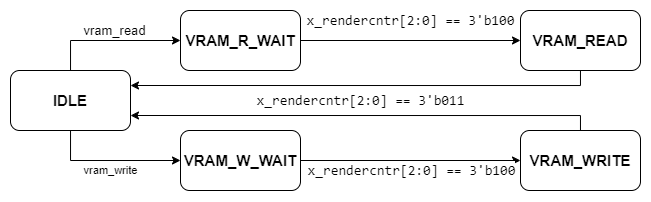
\includegraphics[width=120mm, keepaspectratio]{figures/VRAM-read-write-FSM}
		\caption{CPU-ból ékrekző VRAM írási és olvasási jelek PPU időzítéséhez igazító állapotgép} 
		\label{fig:VRAM-read-write-FSM}
	\end{figure} 	
	
	\subsection{Háttér képalkotást és memória olvasást vezérlő állapot gép}
	
	\Aref{PPU-irodalom} fejezetben olvasottak alapján eredeti PPU kép generálása, két nagyobb egységre bonthatjuk a Háttér és a mozgó csempe elemek sprite-ok generálására. Ebben a fejezetben először az FPGA-ban implementált háttér generálási megoldásokat olvashatjuk.
	
	\begin{figure}[H]
		\centering
		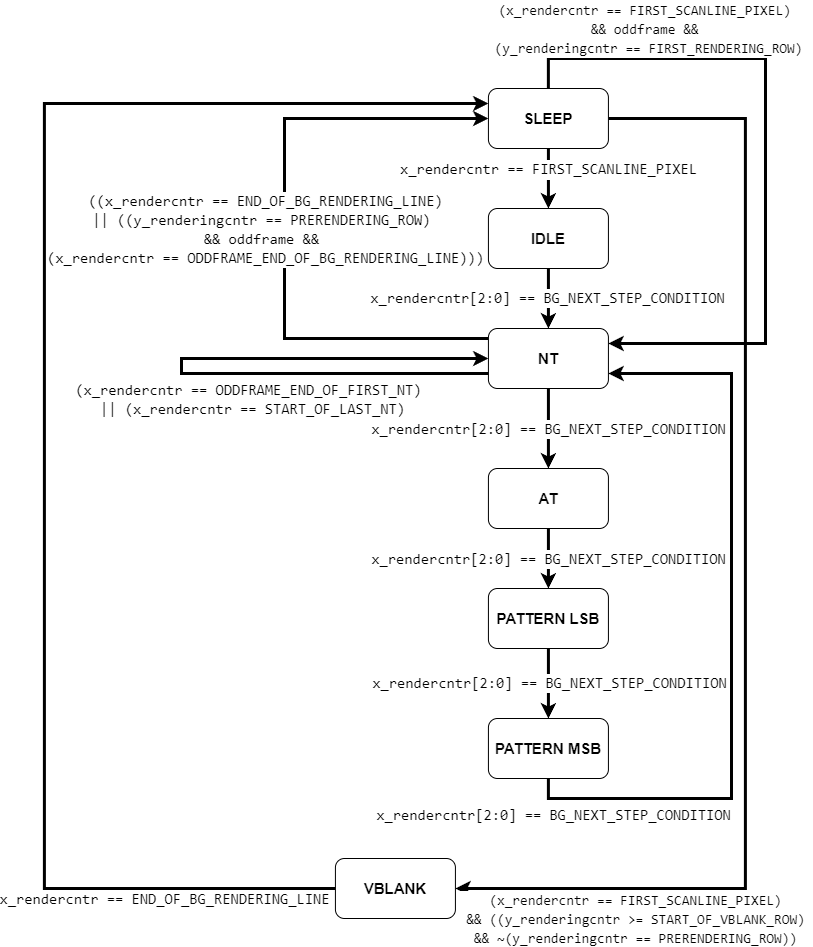
\includegraphics[width=150mm, keepaspectratio]{figures/bg-rendering-FSM}
		\caption{Háttér képalkotás és memória olvasást vezérlő állapotgép} 
		\label{fig:bg-rendering-FSM}
	\end{figure} 
	
	Az FPGA projekt háttér kép alkotását, \aref{fig:bg-rendering-FSM} ábrán látható állapotgép határozza meg. Az állapot átmenetek képzéséhez a chip horizontális és vertikális számlálóit használtam, illetve az eredeti háttér alkotási állapotgépet vettem alapul (\ref{sec:NTSC-PPU-frame}). A chip ismertetése során, már olvashattuk, hogy az eredeti állapotgépben található állapotokban négyszer annyi időt kell tölteni a hardvernek, a VGA jel kiadásának szinkronizálása miatt. Az állapotgépünk hat az eredeti PPU-ban is megtalálható állapotra, és egy SLEEP, blokkoló állapotra bonthatjuk. A SLEEP állapot során a PPU és vele együtt az egész NES hardver egy blokkolt állapotba kerül. Ezalatt az idő alatt a CPU órajel képzését is blokkoljuk, így csak a pixel kétszerezés és a TMDS jelek kiadása zajlik. 
	
	\Aref{fig:bg-rendering-FSM} ábrán látható hat alap állapot, és működése hasonlít az eredeti PPU állapotokhoz (\ref{sec:NTSC-PPU-frame}):
	
	\begin{enumerate}
		\item \emph{Idle:} Minden képgenerálási sor első (nulladik) órajele egy \emph{Idle} állapot, itt a PPU nem végez memória elérést, csak cím regisztereket állít. Minden pártatlan teljes kép generálása során, ez az állapot kihagyásra kerül (helyette az utolsó NT olvasás zajlik le).
		\item \emph{NT, névtáblák olvasása:} Ebben az állapotban kerülnek kiolvasásra a névtábla adatok. A fentebb látható állapotgépben még azt láthatjuk, hogy \aref{sec:NTSC-PPU-frame}-ben is látható módon a 261. sor és a látható képtartomány (0-239 sor) végén a chip még kétszer NT állapotba kerül.
		\item \emph{AT, csempe attribútumok olvasása} Az állapotban a névtábla memóriából a csempéhez tartozó attribútum adatok kiolvasása történik. A későbbiekben ez határozza meg a csempe színeit.
		\item\emph{Pattern LSB (least significant byte):} A névtábla olvasás során megszerzett Pattern csempe cím használatával, egy csempe sor (8 pixel) adatainak, alsó 8 bitjének olvasása történik az állapotban. (\aref{fig:Gumba-tile} képen látható csempe egy sorának alsó bitjei).
		\item \emph{Pattern MSB (most significant byte):} A negyedik állapotban leírt olvasás, befejező lépése történik ebben az állapotban. Tehát a felső 8 bit kiolvasása és mentése. Illetve ennek az állapotnak történik még a vetikális és horizontális VRAM számlálók növelése, \aref{sec:NTSC-PPU-frame} függelékben látható helyeken (vörös négyzetek).
		\item \emph{VBLANK:} Ez az állapot az eredeti PPU vertikális kioltása, a legtöbb játék ezalatt az idő alatt végezte a PPU memória műveletek. Itt hozom létre a PPU státusz regiszter, VBLANK (IRQ) jelét. Ez jelez a NES CPU számára, hogy a VBLANK periódus elkezdődött (szabadon elkezdheti a memória műveleteket a PPU regisztereken keresztül). 
	\end{enumerate} 
	
	A Pattern olvasási állapotok nem csupán a háttér olvasását hanem a Sprite adatok kiolvasását is végzik. \Aref{sec:NTSC-PPU-frame} függelékben láthatjuk is, hogy a 257. órajeltől a 320. órajelig történnek a Sprite csempe adatok olvasásai a következő sorra, a többi részen pedig a háttér adatok kezelése folyik.
	
	A PPU memória területeinek olvasása során, a különböző memória területeket úgy érem el, hogy az adott állapot utolsó órajelére mentésre kerüljön az éppen aktuális adat. Ennek pontos időzítését \aref{code:saving-from-PPU Databus} hardverleírásban olvashatjuk.
	
\begin{lstlisting}[caption={Az állapotgép alapján az adatok mentét vezérlő jelek}, label={code:saving-from-PPU Databus}, style=prettyverilog]
assign nametable_read = (bgrender_state == NT) & (x_rendercntr[2:0] == 3'b011);
assign attribute_read = (bgrender_state == AT) & (x_rendercntr[2:0] == 3'b011);
assign bg_lsb_read = (bgrender_state == BG_LSB) & (x_rendercntr[2:0] == 3'b011);
assign bg_msb_read = (bgrender_state == BG_MSB) & (x_rendercntr[2:0] == 3'b011);\end{lstlisting}
	
	\Aref{sec:NTSC-PPU-frame} függelékben a 241. sorban látható VBLANK jel elő állítása során különösen figyelni kellet az időzítésre. Mivel ennek a jelnek a hatására képződik a 6502-es CPU felé az NMI (non maskable interupt) megszakítás (\aref{code:vblank-set} IRQ), amelynek pontos lefutása elengedhetetlen a játékok emulálása szempontjából. Ez a megszakítás tartalmazza általában azt a programkódot, amely a név memória területek frissítésért felelős. A pontos időzítést az FPGA projektben, egy két bites léptető regiszter használatával állítom be, ezt és a vezérlő jelek képzését \aref{code:vblank-set} hardverleírásban olvashatjuk.       
		
\begin{lstlisting}[caption={VBLANK vezérlőjelek képzése és az NMI (IRQ) jel előállítása}, label={code:vblank-set}, style=prettyverilog]
//Driving the interupt flag
reg  interrupt_flag;
wire interrupt_clr;
always @ (posedge clk) 
begin
	if (rst || interrupt_clr || (status_rd && ph2_falling))
		interrupt_flag <= 1'b0;
	else
		if (vblank_set[2] && vblank[1])
			interrupt_flag <= 1'b1;
end
//NMI towards cpu
always @ (posedge clk) 
begin
	if (rst)
		irq <= 1'b0;
	else
		irq <= interrupt_flag & vblank_irq_enable; 
end
	
// vblank set signals
assign vblank_set[0] = (x_rendercntr == (FIRST_SCANLINE_PIXEL +  0)) & (y_renderingcntr == V_BLANK_BEGIN);
assign vblank_set[1] = (x_rendercntr == (FIRST_SCANLINE_PIXEL +  4)) & (y_renderingcntr == V_BLANK_BEGIN);
assign vblank_set[2] = (x_rendercntr == (FIRST_SCANLINE_PIXEL + 12)) & (y_renderingcntr == V_BLANK_BEGIN);

//Indicates the end of the VBLANK period.
assign vblank_clr    = (x_rendercntr == FIRST_SCANLINE_PIXEL +  4) & (y_renderingcntr == PRERENDERING_ROW);
assign interrupt_clr = (x_rendercntr == FIRST_SCANLINE_PIXEL + 12) & (y_renderingcntr == PRERENDERING_ROW);\end{lstlisting}
	
	\subsection{Mozgó csempe elemek "Sprite" képalkotás}
	\label{sec:fpga-sprite-rendering}

	A PPU-ban található képalkotás második rétege a mozgó csempe elemek kiolvasása és feldolgozása a OAM memóriából. Az eredeti hardver felépítéséről részletesen olvashatunk \aref{sec:OAM-memory} fejezetben, az itt olvasottak alapján alakítottam ki a OAM memóriákat is az FPGA modul során. 
	
	Az elsődleges és a másodlagos OAM memóriát is Distributed memória ként hoztam létre a lehető leggyorsabb olvasási idő miatt. A Distributed memória az FPGA LUT-jából közvetlenül leképeződő memória, általában olyan helyeken szokták alkalmazni ahol kevés adatot kell tárolni, és gyors elérésre van szükségünk (azonnal elérhető). A mi felhasználásunk során elengedetlen a késleltetés mentes adat kiolvasás, mert a háttér állapotgépet és a sprite állapotgépet szinkronizálni kell a Pattern adatok olvasása miatt.
	
	Az Sprite képalkotásban fontos szerepe van a DMA-ból érkező adat időben történő mentésének és ezzel párhuzamosan egy olyan elsődleges OAM RAM címzésnek, amely jól lekezeli a DMA-ból érkező adatokat és a sprite állapotgépben a másodlagos OAM memória feltöltését is. 
	
	A címképzésnek két fő módja van. Az első mód során, az elsődleges RAM címzését két mozgó számlálóval címezzük meg, m és n. M a négy bájtos sprite adatokon halad végig, amíg az n pedig a 64 sprite-on halad végig, ezeknek a számlálóknak az időzítését a sprite állapotgéphez kötöttem. Ezt a címzési módot használom a másodlagos OAM memória töltése során, tehát az aktív spritok keresésére. A második mód pedig a DMA működése során aktív cím, ez egy egyszerű fölfelé számláló, amely a CPU-tól kapja kezdő címét, az oam címregiszter írása során.
	
	Az így létrejövő két címet megfelelően multiplexálva kapjuk meg az elsődleges OAM memória címzését. A cím képzését és az elsődleges OAM írását és olvasását \aref{code:Primary-oam} hardverleírásban olvashatjuk.

\begin{lstlisting}[caption={Az elsődleges OAM RAM írása és olvasása}, label={code:Primary-oam}, style=prettyverilog]
(* ram_style = "distributed" *)
reg  [7:0]  pri_oam [255:0];
reg  [7:0]  pri_oam_addr;
wire [1:0]  pri_oam_addr_sel;
wire [7:0]  pri_oam_dout = pri_oam[pri_oam_addr];

always @(*) 
begin
	case (pri_oam_addr_sel)
		2'b01:   pri_oam_addr <= {n_cnt, m_cnt};
		2'b11:   pri_oam_addr <= {pri_oam_addr_cnt[7:3], n_cnt[0], m_cnt}; 
		default: pri_oam_addr <= pri_oam_addr_cnt; 
	endcase    
end

always @(posedge clk) 
begin
	if (oam_data_wr)
		pri_oam[pri_oam_addr] <= slv_mem_din;    
end\end{lstlisting} 

	Az sprite képgenerálás állapotgépének fontos eleme még, a következő sorban aktív sprite-ok detektálásáért felelős hardveres egység \ref{code:Sprite-in-range}. Ennek alapja, hogy az állapotgép alapján képzett vezérlőjellel (oam\_temp\_reg\_wr) elmentjük az éppen aktív OAM sprite vertikális pozíció értékét és az éppen aktív sor értékből kivonva egy vertikális különbség értéket képzünk. Ezt vizsgálva a 8x8 és 8x16-os spritok esetére, detektálhatjuk, hogy az éppen aktív sprite a következő sorban megjelenik-e. Abban az esetben ha találtunk egy megjelenítendő sprite-ot akkor az állapotgép alapján (\ref{fig:sprite-rendering-FSM}) továbblépve ezt mentjük a másodlagos memóriába, vagy még egyel növeljük a túlcsordulás jelzőt. 

\begin{lstlisting}[caption={A következő kép generálási sorban aktív sprite-ok jelzése}, label={code:Sprite-in-range}, style=prettyverilog]
reg  [8:0]  y_diff_reg1;
wire      sprite_in_range = (sprite_size) ? (y_diff_reg1[8:4] == 5'd0) : (y_diff_reg1[8:3] == 6'd0);


// if I subtract from scanline cntr - tile_addr then check the upper bits of y_diff_reg to be zero then we have a sprite in range
always @(posedge clk) 
begin
	if (rst)
		y_diff_reg1 <= 9'd0;
	else
		if (oam_temp_reg_wr)
			y_diff_reg1 <= scanline_cnt - {1'b0, pri_oam_dout};    
end\end{lstlisting}

	\begin{figure}[H]
	\centering
	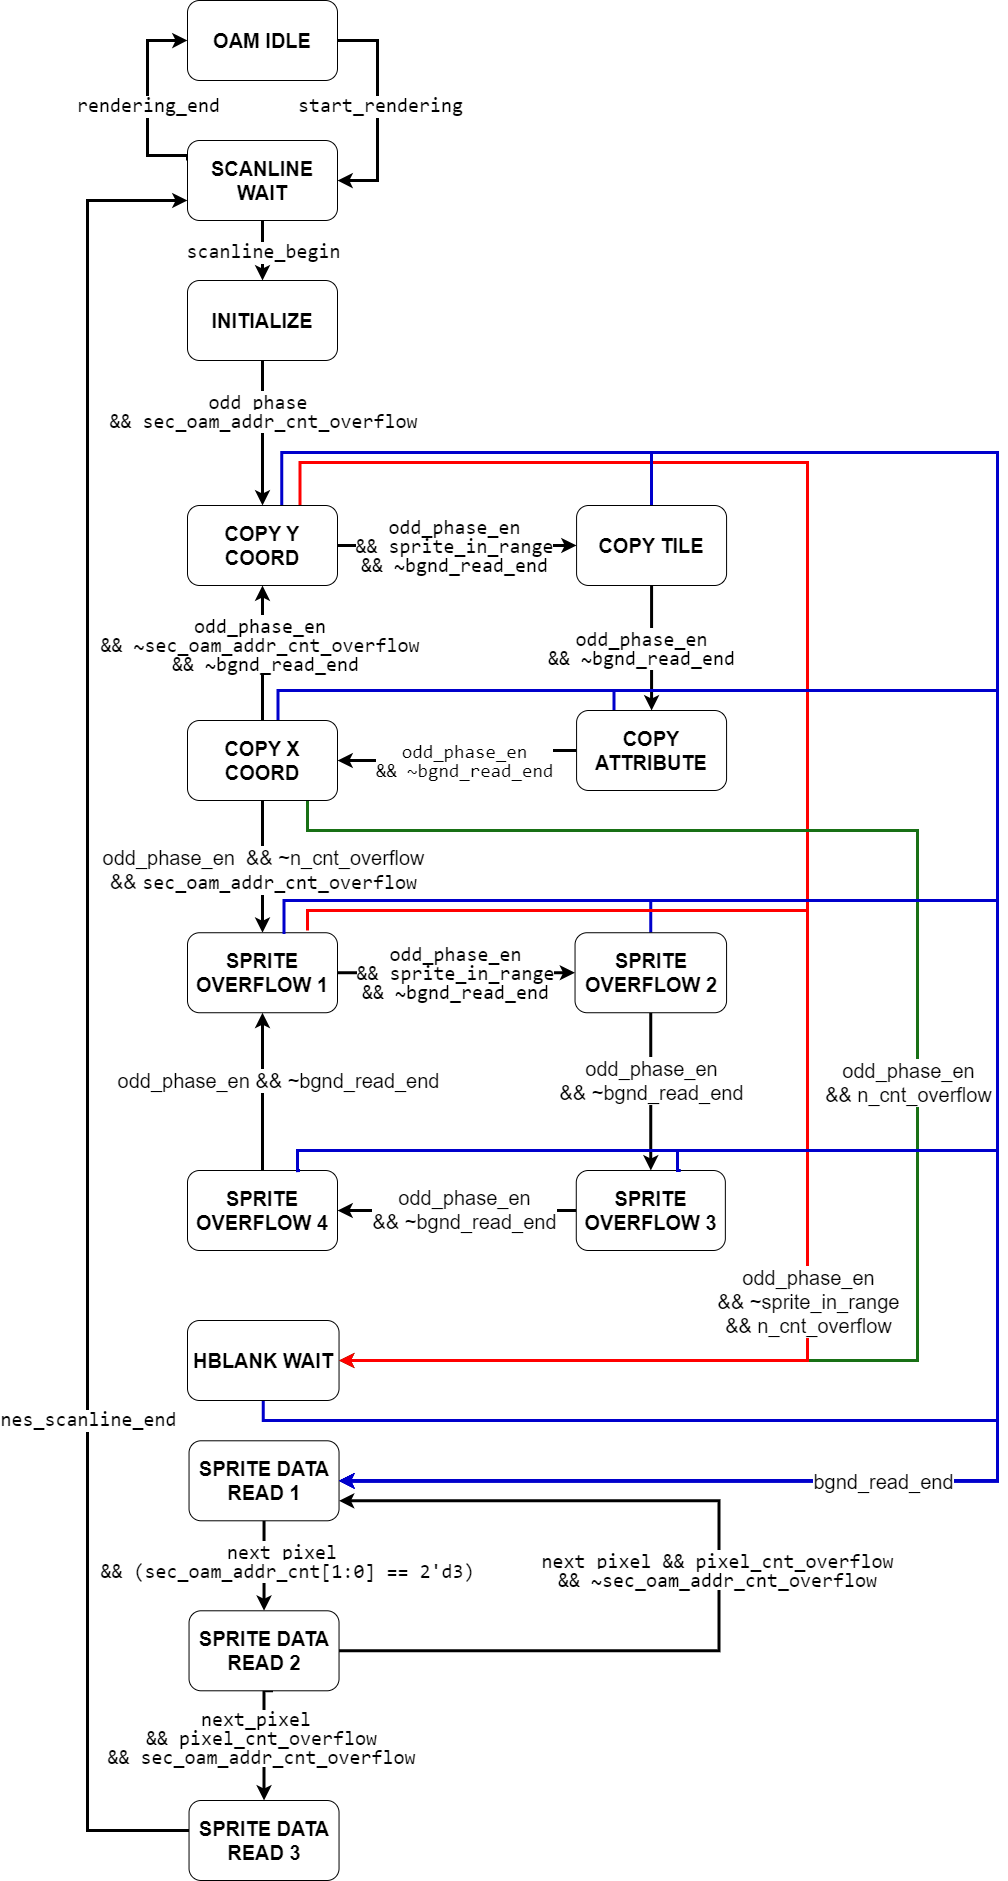
\includegraphics[width=125mm, keepaspectratio]{figures/sprite-rendering-FSM-v3}
	\caption{Sprite képalkotás és memória olvasást vezérlő állapotgép} 
	\label{fig:sprite-rendering-FSM}
	\end{figure} 

	Az állapotgép teljes körű megértéséhez elengedetlen, hogy az eredeti hardvert megértsük. Az eredeti sprite feldolgozás menete négy fő részre bontható, ez \aref{sec:NTSC-PPU-frame} függelékben is látható. 	
	
	\begin{enumerate}
		\item A nyolc előző sorban mentet sprite törlése (1-64 órajel) \Aref{fig:sprite-rendering-FSM} állapotgépben ez az IDLE állapot.
		\item Az elsődleges OAM RAM, végig olvasása aktív sprite-okat keresve. Minden egyes páratlan órajel során olvassa az adatokat, a párosok alatt pedig írja őket a memória területre. Ha aktív sprite-ot találunk a négy bájtját mentjük a másodlagos OAM RAM-ba. (65-256 órajel) \Aref{fig:sprite-rendering-FSM} állapotgépben ez sorrendben az Y koordináta másolása, csempe cím másolása, csempe attribútum másolása és X koordináta másolása állapotoknak felel meg.
		\item Ha megtalált nyolc aktív sprite-ot, akkor tovább keres a sorban hátha túlcsordulást érzékel. Itt a memória olvasásban egy hardveres hiba található, mivel ha talált egy extra aktív spriteot is akkor a következő sprite-ok Y koordinátája helyett a sorban következő bájtot (csempe cím) vizsgálja a rendszer. Ha ezt követően is talál még egy aktív sprite-ot, akkor pedig az ezt követő sprite bájtokat kezdi el vizsgálni (csempe attribútum). (65-256 órajel) \Aref{fig:sprite-rendering-FSM} állapotgépben ez a négy túlcsordulási állapotnak felel meg.
		\item Végül az utolsó lépésben az aktív sprite adatok kiolvasása és mentése következik. (257-320 órajel) \Aref{fig:sprite-rendering-FSM} állapotgépben ez a három sprite adat olvasási állapotnak felel meg.
	\end{enumerate}

	\Aref{fig:sprite-rendering-FSM} ábrán látható állapotgép két extra állapottal bővül ki az FPGA rendszer szinkronizációja miatt. Az első két állapot (OAM IDLE és SCANLINE WAIT) a VGA jel generálás alatti IDLE állapotot reprezentálja (hasonlóan \aref{fig:bg-rendering-FSM} SLEEP állapotához). Illetve a HBLANK WAIT állapot amely a túlcsordulás figyelést követően szinkronizálja az állapot gép működését.

	Az állapotgép negyedik szakasza teljes mértékben szinkron működik a háttér képalkotást vezérlő állapotgép Pattern adat olvasásával. Az innen kiolvasott két bájtos csempe adatokat egy-egy pufferbe mentjük, ha kevesebb mint 8 aktív sprite van egy sorban akkor a fennmaradó puffer területek nullás értéket kapnak. A pufferek léptető regiszterként tárolják a csempe adatokat és figyelik a képalkotás horizontális számlálóját, ha az aktuális sprite X koordinátája megegyezik a sor indexel, akkor elkezdődik a 8 pixelnyi képadat léptetése és kiadása. Ha a $sprite\_clipping$ jel aktív akkor az első csempe oszlop idő tartalma alatt nem történhet mozgó csempe megjelenítés, tehát ezeknek a sprite-oknak az értéke nullázódik. Ennek segítségével tudunk szép folyamatos bal oldali görgetést létrehozni.
	
	Végül a pufferekből érkező sprite, pixeladati között meghatározzuk a prioritási sorrendet és a nagyobb prioritással rendelkező pixel adatait adjuk ki a sprite képalkotási modulból. A prioritást az elsődleges OAM memóriában való elhelyezkedés határozza meg, a nulladik sprite nak van a legnagyobb prioritása és a 63.-nak pedig a legkisebb (tehát minél előbb kerül a másodlagos OAM-ba a sprite annál nagyobb a prioritása).
	
	A játékok hibátlan emulálása szempontjából elengedhetetlen még a $sprite_0\_hit$ vezérlő jel pontos elő állítása. Ha ezt nem pontosan hozzuk létre egyes játékok, többek között a Super Mario Bros. a kezdő képernyőn ragad és nem kezd el futni a teljes szoftver (valószinüleg egy várakozó állapotban ragad). A jel egyik komponensét a $sprite_0\_visible$ jelet, a sprite képalkotást vezérlő modulon belül, \aref{code:sprite0-visible} hardverleírásban látható módon hozom létre. A végső $sprite_0\_hit$ jel pedig a logikai és kapcsolata a $sprite_0\_visible$, $visible\_bg\_pixel$ és a $sprite_0\_check$ jeleknek. A látható háttér pixel a nem átlátszó háttér pixelek során aktív, a $sprite_0\_check$ pedig azt vizsgálja, hogy a horizontális képalkotás elért-e a 255. pixelig. 

\begin{lstlisting}[caption={A $sprite_0\_visible$ vezérlő jel elő állítása}, label={code:sprite0-visible}, style=prettyverilog]
reg [1:0] sprite0_in_range;
assign sprite0_visible = sprite0_in_range[1] & |sprite_pixel[1:0] & ~(~sprite_enabled | (first_column & ~no_sprite_clip)); 

always @(posedge clk) 
begin
	if (rst)
		sprite0_in_range <= 2'd0;
	else
		if (scanline_begin)
			sprite0_in_range <= {sprite0_in_range[0], 1'd0};
	else
		if (odd_phase_en && (oam_state == OAM_COPY_X_COORD) && (n_cnt == 6'd0))
			sprite0_in_range <= {sprite0_in_range[1], 1'b1};
end\end{lstlisting} 

	\subsection{PPU adatbusz és memória elérése}
	
	A PPU működéséhez elengedetlen a VRAM cím regiszterének képzése is, ennek felépítése két rétegből tevődik össze (az eredeti PPU mintájára). Az első réteg \aref{sec:CPU-databus-ppu_reg} fejezetben leírtak alapján, a CPU adatbuszról érkező regiszter írások hatására, egy regiszterbe menti a VRAM címet, ennek az pontos elérése látható \aref{fig:2000-2005-2006-ppu-reg-writes} ábra t regiszter módosulásin. A második réteg pedig a képgenerálás során képződő számlálást és a soron kívüli regiszter töltéseket és fölfelé számolásokat foglalja magába (\aref{fig:2000-2005-2006-ppu-reg-writes} ábrán v regiszternek felel meg).
	
	A cím számláló réteg különleges olyan szempontból, hogy megkülönböztet két fajta felfelé számolási sorrendet. Az első a standard számlálás, amikor a cím két része horizontális és vertikális külön-külön számolnak felfelé mint két különálló regiszter. Ezt a számlálási módot használja a PPU \aref{sec:NTSC-PPU-frame} függelékben látható vörös pixelek megvalósítása során, tehát az általános képgenerálás során. A második számlálási mód pedig amikor a VRAM írása vagy olvasása hatására egy felfelé számlálás történik, itt a teljes VRAM címregiszter számol fölfelé 1-et vagy 32-t a (a számlálási mód függvényében). 
	
	\begin{figure}[H]
	\centering
	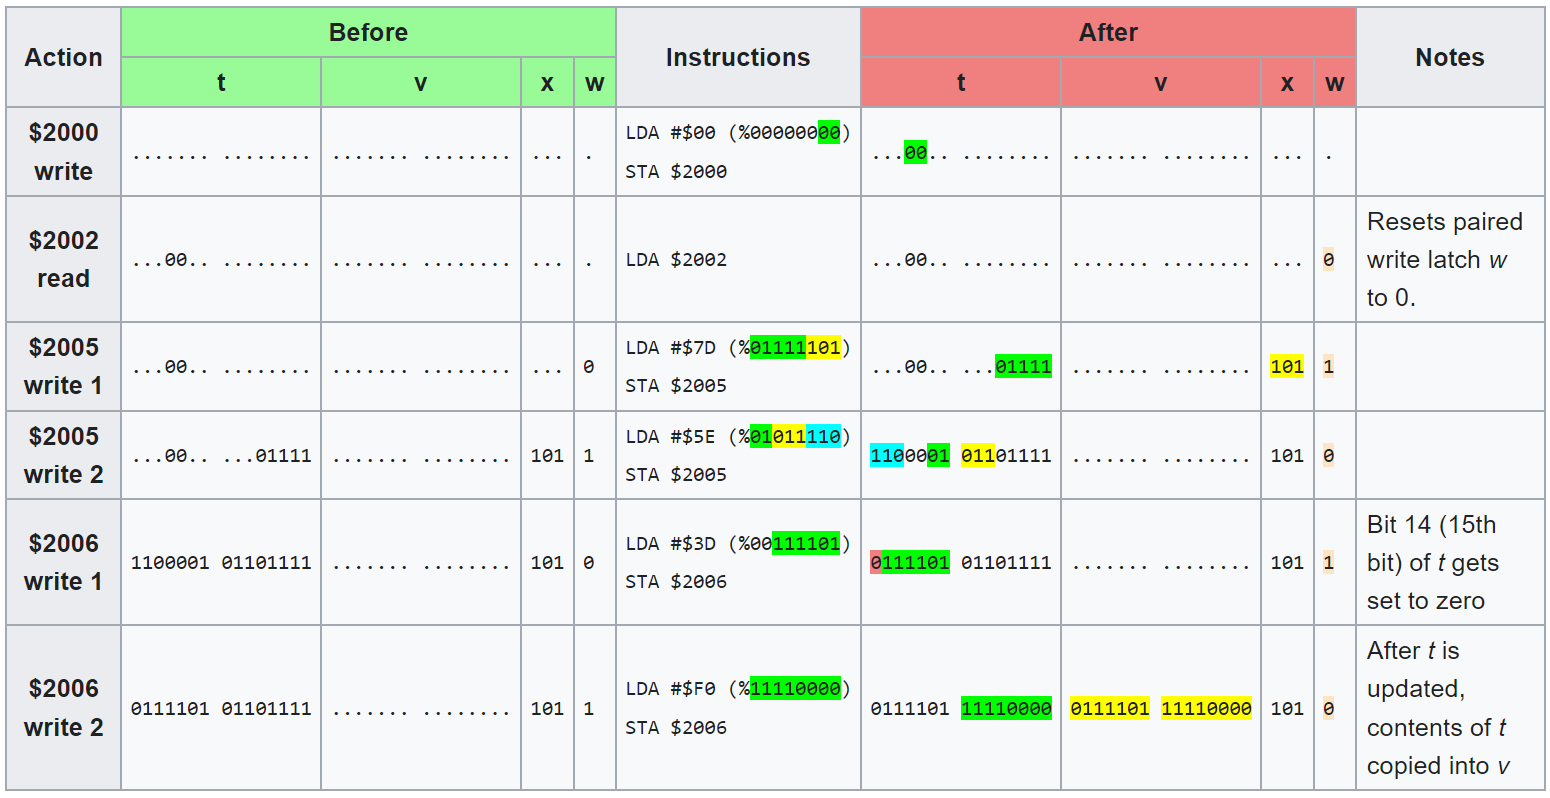
\includegraphics[width=150mm, keepaspectratio]{figures/2000-2005-2006-ppu-reg-writes}
	\caption{VRAM cím regiszter értékadása (eredeti PPU)} 
	\label{fig:2000-2005-2006-ppu-reg-writes}
	\end{figure} 
	
	A \ref{sec:NT-AT-mirroring} fejezetben leírtak alapján, a VRAM címszámláló regiszterekből hozom létre a név tábla és attribútum tábla címeit. Majd az NT  állapotban kiolvasott pattern cím adatok segítségével létrehozom a háttér csempeadatok olvasási címét. A sprite állapot gépből érkező adatok alapján a $sprite\_size$-nak megfelelően állítok elő pattern címeket a 8 aktív csempeadat kiolvasása számára. A pontos címképzéseket \aref{code:VRAM-addr} hardverleírásban olvashatjuk.
	
\begin{lstlisting}[caption={VRAM cím képzése a számlálókból és az állapotgépek alapján}, label={code:VRAM-addr}, style=prettyverilog]
wire [13:0] ppu_nt_addr = {2'b10, v_cnt, h_cnt, vt_cnt, ht_cnt};
wire [13:0] ppu_at_addr = {2'b10, v_cnt, h_cnt, 4'b1111, vt_cnt[4:2], ht_cnt[4:2]};
wire [13:0] bg_lsb_addr = {1'b0, background_pattern_sel, tile_index_reg, 1'b0, fv_cnt};
wire [13:0] bg_msb_addr = {1'b0, background_pattern_sel, tile_index_reg, 1'b1, fv_cnt};

assign sprite_lsb_addr = (~sprite_size) ? ({1'b0, sprite_pattern_sel, sprite_tile_index, 1'b0, sprite_range[2:0]}) : ({1'b0, sprite_tile_index[0], sprite_tile_index[7:1], sprite_range[3], 1'b0, sprite_range[2:0]});
assign sprite_msb_addr = (~sprite_size) ? ({1'b0, sprite_pattern_sel, sprite_tile_index, 1'b1, sprite_range[2:0]}) : ({1'b0, sprite_tile_index[0], sprite_tile_index[7:1], sprite_range[3], 1'b1, sprite_range[2:0]});\end{lstlisting}

	A PPU (mester) adatbusz cím regiszterének meghajtása során, figyelembe kell vennünk azt, hogy ha a chipen bármilyen VRAM elérést hajtanak végre, akkor a címregisztert ne a VRAM cím számláló rétegéből határozzuk meg, hanem egy extra regiszteren a $vram\_addr\_reg$-en keresztül adjuk ki, ezzel késleltetve a címünket egy órajellel. Ez, az eredeti NES PPU-ban is, egy hardveres hiba volt, amire játékok építettek is (például a Super Mario Bros.). Abban az esetben is, ha a háttér vagy a sprite képalkotás nincs kiválasztva tehát $ppu\_enable$ inaktív, automatikusan a késleltetett VRAM címet kell kiadni. 
	
	A végső cím kimenetet még szinkronizálnunk kell a chip többi részéhez, erre szolgál az $addr\_reg\_ld$ jel. Az adatbusz címregiszterének képzését \aref{code:PPU-master-databus-addr} hardverleírásban láthatjuk részletesebben.

\begin{lstlisting}[caption={PPU master adatbusz címregiszterének meghajtása és időzítése}, label={code:PPU-master-databus-addr}, style=prettyverilog]
wire vram_address_sel = (vram_state_machine_sel == VRAM_RD_WAIT) || (vram_state_machine_sel == VRAM_WR_WAIT);
wire [7:0] ppu_address_sel;
wire addr_reg_ld = (x_rendercntr[2:0] == 2'b100);

assign ppu_address_sel [0] = vram_address_sel;
assign ppu_address_sel [1] = (bgrender_state == NT);
assign ppu_address_sel [2] = (bgrender_state == AT);
assign ppu_address_sel [3] = (bgrender_state == BG_LSB) & sprite_read;
assign ppu_address_sel [4] = (bgrender_state == BG_MSB) & sprite_read;
assign ppu_address_sel [5] = (bgrender_state == BG_LSB) & ~sprite_read;
assign ppu_address_sel [6] = (bgrender_state == BG_MSB) & ~sprite_read;
assign ppu_address_sel [7] = ppu_enable;

always @(posedge clk) 
begin
	if (rst)
		ppu_mem_addr <= 14'd0;
	else
		if (addr_reg_ld)
			case (ppu_address_sel)
				8'b10000010 : ppu_mem_addr <= ppu_nt_addr;
				8'b10000100 : ppu_mem_addr <= ppu_at_addr;
				8'b10001000 : ppu_mem_addr <= sprite_lsb_addr;
				8'b10010000 : ppu_mem_addr <= sprite_msb_addr;
				8'b10100000 : ppu_mem_addr <= bg_lsb_addr;
				8'b11000000 : ppu_mem_addr <= bg_msb_addr;
				default		: ppu_mem_addr <= vram_addr_reg;
			endcase
end\end{lstlisting}

	\subsection{A PPU részéről történő kép generálás működése}
	
	A háttér állapot gép futása során kiolvasott csempe adatok feldolgozása hasonlít a sprite pixel feldolgozásra, azzal a különbséggel, hogy ennek folytonosan futnia kell a háttér képalkotás ideje alatt. Ezt az FPGA modulon belül egy különleges hardveres elemmel egy LUT-ban szintetizálódó léptető regiszterrel SRL-el (shift register LUT) oldottam meg. Ennek az elemnek a különbsége, hogy a teljes regiszter töltése nem engedélyezett csak a regiszterek bitszélességével történő léptetéses töltés. Ennek előnye hogy könnyen össze szinkronizálható a háttér csempék két bájt-ja (mivel az LSB és MSB bájtok bit párjai alkotják a háttér egy pixelét) és kimenetként pedig bármelyik bit választható. A kimenet választás azért fontos, mert a görgetés során egy csempét pixelekként szeretnénk ki görgetni a megjelenített kép tartományból és ennek segítségével az összes párhuzamosan működő regiszter aktív kimeneti bitje egyszerre módosítható. Ilyen SRL-t használtam a csempe attribútumának megjelenítésére is. Ezt az adatfeldolgozó láncot olvashatjuk \aref{code:SRL-shiftregs} hardverleíró részletben.
	
	\begin{figure}[H]
	\centering
	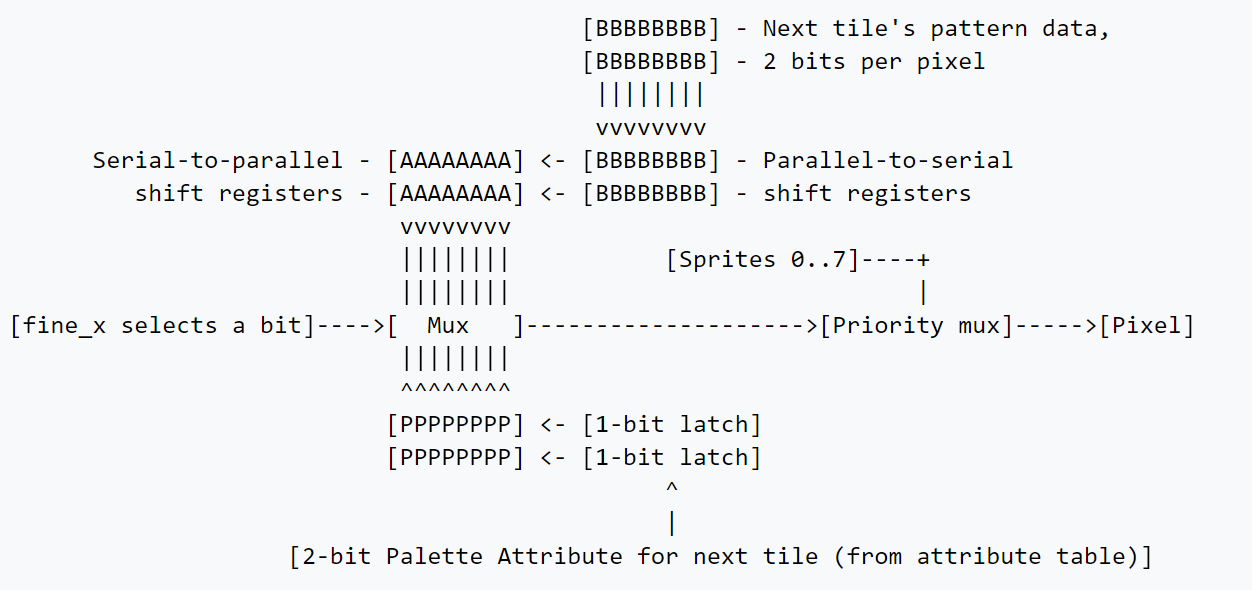
\includegraphics[width=120mm, keepaspectratio]{figures/NES-render-chamber}
	\caption{A NES PPU-jának pixel feldolgozó egysége} 
	\label{fig:NES-render-chamber}
	\end{figure} 
	
	Az állapotgépek pixel feldolgozó egységei és működése nagyban hasonlít az eredeti hardver felépítésére, ezt \aref{fig:NES-render-chamber} ábrán láthatjuk. A PPU két állapot gépe során kapott pixel adatok összefűzésének és feldolgozásának három fő fázisa van.
	
	\begin{enumerate}
		\item \emph{Prioritás vizsgálat, végső pixel meghatározása:} A sprite képalkotás kétféle képen történhet, a mozgó csempe elem kerülhet a háttér elé, illetve a háttér mögé erről a csempe prioritása dönt(ha: 1 akkor a háttér mögé kerül a mozgó elem), ennek segítségével alkották meg a játékfejlesztők például a Mario húsevő növényeit. A pixel kiválasztás során még figyelembe kell venni hogy a háttér pixel átlátszó-e, ebben az esetben mindenképpen a sprite képkockáját válasszuk. Ezt a kiválasztási folyamatot láthatjuk \aref{code:SRL-shiftregs} hardver leíró részlet alján.
		\item \emph{Paletta lookup táblázat:} Az így kiválasztott pixel egy paletta címet képez, a NES CPU-ja által töltött Paletta lookup táblázatban. Ennek működéséről olvashatunk \aref{sec:Pattern-tables-and-palettes} fejezet során. Az FPGA-ban történő megvalósításban itt is Distributed memóriát használtam, a késleltetés mentes olvasás miatt. A helyes emulálás miatt különösen figyelnünk kell a memória területek helyes tükrözésére, ha ezt nem jól implementáljuk eggyes játékok színei nagyban eltérhetnek az eredetitől, például a Mario háttere kék helyett fekete lesz. Ennek helyes implementálását olvashatjuk \aref{code:palette-mirroring} hardver leírásban. Ha a $BG\_clipping$ jel aktív és az első csempe oszlopban vagyunk, vagy a PPU várakozó állapotban van (\ref{fig:bg-rendering-FSM} SLEEP állapota), akkor automatikusan egy fekete pixel értékével helyettesítjük a palettából olvasott címet.
		\item \emph{RGB blokk ROM:}Az FPGA implementálás során a paletta memóriából kiolvasott színérték egy címként értelmeztem és készítettem egy RGB adatokkal előre feltöltött ROM-ot, amely a címhez a megfelelő 24 bites RGB értéket rendeli. Itt még figyelembe vettem a NES képalkotást befolyásoló két funkciót. Az első a monokróm mód, amely fekete fehér képalkotást tesz lehetővé. Ezt úgy implementáltam, hogy a palettából kiolvasott cím, HUE értékének megfelelő biteket nullával helyettesítem. A második ilyen mód pedig, a szín kiemelés (a PPU képes volt, adott színek kiemelésére és a többi szín elsötétítésére). Ezt a tulajdonságot egyszerűen úgy implementáltam, hogy a Paletta ROM címébe beletartoznak az $emphesize\_r / -\_g / -\_b$ jelek, így egy kicsit nagyobb blokk ROM-ot képezve a hardverben.
	\end{enumerate} 
	
\begin{lstlisting}[caption={Pixel adat feldolgozó SRL léptető regiszterek}, label={code:SRL-shiftregs}, style=prettyverilog]
//LSB of backgorund pixel
reg [7:0] bg_lsb_buff_reg;
always @ (posedge clk) 
begin
	if (rst)
		bg_lsb_buff_reg <= 8'd0;
	else
		if (bg_msb_read)
			bg_lsb_buff_reg <= bg_lsb_reg; // shift reg
		else if ((x_rendercntr[1:0] == 2'b11) && (x_rendercntr > START_OF_SHIFT) && (x_rendercntr <= END_OF_SHIFT) && ~(bgrender_state == VBLANK))
			bg_lsb_buff_reg <= {bg_lsb_buff_reg[6:0], 1'b0}; 
end
reg [7:0] shr_lsb_render = 8'd0;
wire	  bg_lsb_out;  
always @(posedge clk) 
	if ((x_rendercntr[1:0] == 2'b11) && (x_rendercntr > START_OF_SHIFT) && (x_rendercntr <= END_OF_SHIFT) && ~(bgrender_state == VBLANK))
		shr_lsb_render <= {shr_lsb_render[6:0], bg_lsb_buff_reg[7]};
assign bg_lsb_out = shr_lsb_render[~fh_reg];
//MSB of background pixel
reg [7:0] shr_msb_render = 8'd0;
wire	  bg_msb_out;  
always @(posedge clk) 
	if ((x_rendercntr[1:0] == 2'b11) && (x_rendercntr > START_OF_SHIFT) && (x_rendercntr <= END_OF_SHIFT) && ~(bgrender_state == VBLANK))
		shr_msb_render <= {shr_msb_render[6:0], bg_msb_reg[7]};
assign bg_msb_out = shr_msb_render[~fh_reg];

//0 bit of attribute
reg [7:0] shr_attr0_render = 8'd0; 
always @(posedge clk) 
	if ((x_rendercntr[1:0] == 2'b11) && (x_rendercntr > START_OF_SHIFT) && (x_rendercntr <= END_OF_SHIFT) && ~(bgrender_state == VBLANK))
		shr_attr0_render <= {shr_attr0_render[6:0], tile_attr_reg_saved[0]};
wire shr_attr0_out = shr_attr0_render[~fh_reg];
//1 bit of attribute
reg [7:0] shr_attr1_render = 8'd0; 
always @(posedge clk) 
	if ((x_rendercntr[1:0] == 2'b11) && (x_rendercntr > START_OF_SHIFT) && (x_rendercntr <= END_OF_SHIFT) && ~(bgrender_state == VBLANK))
		shr_attr1_render <= {shr_attr1_render[6:0], tile_attr_reg_saved[1]};
wire shr_attr1_out = shr_attr1_render[~fh_reg];

//pixel output
reg [3:0] bg_pixel;
always @(posedge clk) 
begin
	if (rst)
		bg_pixel <= 4'b0;
	else
		bg_pixel <= {shr_attr1_out, shr_attr0_out, bg_msb_out, bg_lsb_out};		
end
wire [4:0] palette_addr = 	(sprite_priority & visible_bg_pixel) ? ({1'b0, bg_pixel}) : ({1'b1, sprite_pixel});\end{lstlisting}

\begin{lstlisting}[caption={A paletta címek tükrözése}, label={code:palette-mirroring}, style=prettyverilog]
wire [4:0] palette_ram_nt_addr_mirrored = {vram_addr_cnt[4] & |vram_addr_cnt[1:0], vram_addr_cnt[3:0]};									
wire [4:0] palette_ram_addr_mirrored = {palette_addr[4] & |palette_addr[1:0], palette_addr[3:0]};\end{lstlisting}

	\subsection{A VGA képalkotás}
	
	A PPU véső hardveres eleme, az RGB adatokat tároló és megjelenítő VGA modul, ennek felépítését láthatjuk \aref{fig:vga-rendering-top} ábrán. 
	
	\begin{figure}[H]
		\centering
		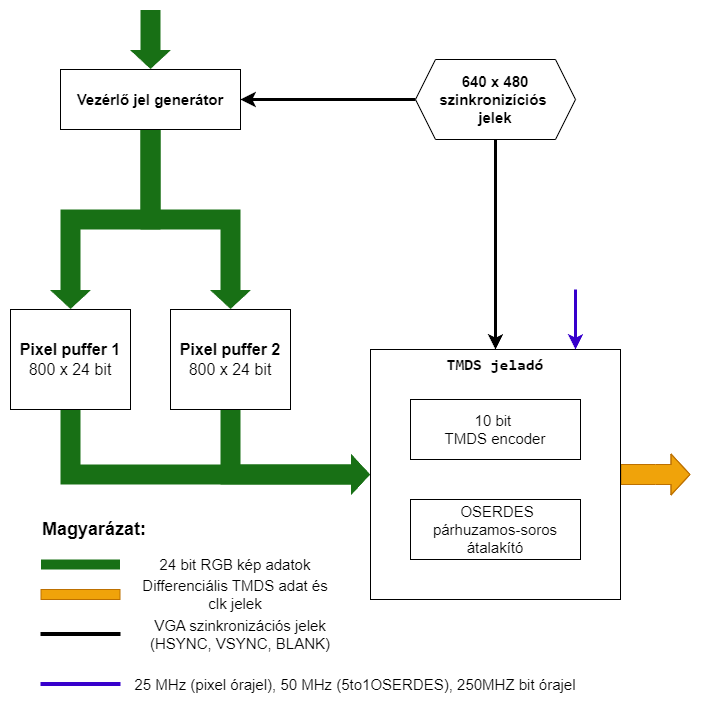
\includegraphics[width=120mm, keepaspectratio]{figures/vga-top-diagram}
		\caption{VGA top modul blokkvázlata} 
		\label{fig:vga-rendering-top}
	\end{figure} 

	A PPU bemutatása során \aref{sec:PPU-FPGA} már bemutattam a chip áttervezésének, alap ötletét miszerint a PPU egy képalkotási sora alatt 1600 órajel, a pixeleket minden második órajelben mintavételezve megkapom a 800 pixel széles vga képem egy sorát. Majd a következő kép sor mintavételezése alatt, az előző sort kétszer kiadva hozzuk létre az eredeti NES pixelek nagyítását és kapjuk meg a 640x480-as VGA képalkotás két sorát. Így a VGA kép egy sor késésben lesz a PPU képalkotáshoz képest, viszont helyes indulási időzítések mellet ez nem észrevehető. Puffereket egy-egy kilobájtnyi blokk RAM-ként alakítottam ki a VGA modulon belül, mivel az így kiolvasott adatok egy órajelnyi késleltetése nem okoz semmilyen extra csúszást a VGA időzítésben. Ez a dupla pufferelés látható \aref{fig:vga-rendering-top} ábrán is, természetesen ezek közül egyszerre csak az egyik puffer kimenet aktív és a két pufferkimenetei dinamikusan váltják egymást a PPU-ban történő képsor növekedésével.
	
	A TMDS jeladó és a pufferek töltésének kezdetét vezérlő jelek időzítése különösen fontos, hiszen ezek segítségével vagyunk képesek a PPU aktív képtartományát pozicionálni a VGA pixel sor közepére. A pixel kétszerezést követően a PPU aktív képtartománya 512 pixel órajelig tart. Tehát A helyes időzítéshez 64 pixel órajelig fekete pixelt kell a TMDS adónak venni, majd következik az 512 pixelnyi aktív képkocka végül pedig 224 képkockányi fekete kocka, ez a tartomány tartalmazza a horizontális kioltási területeket is. Ennek a képkocka aránynak a kialakítása határozza meg \aref{fig:bg-rendering-FSM} háttér állapotgépben a SLEEP állapotból történő kilépést, illetve a puffer töltési idő kezdetének meghatározásával még finom hangolható a kép pontos beállítása. Ahhoz, hogy a kezdetektől fogva helyes kép jelenjen meg a monitorunkon, a VGA szinkronizálási jelek generálását is be kellet késleltetnem a pre-rendering sor, és az első puffer feltöltésének idő tartalmával. Ezt egy egyszerű, csak reset jelre nullázódó számláló segítségével oldottam meg, amely 3201 pixel órajelet (két teljes PPU sor + 1 pixel órajel) követően engedélyezi a generálást. A szinkronizációs jelek pontos időzítése a pixel órajelhez képet \aref{code:vga-timing} hardverleírásban látható. 
	
\begin{lstlisting}[caption={A képgenerálás időzítési paraméterei}, label={code:vga-timing}, style=prettyverilog]
localparam H_BLANK_BEGIN     = 10'd639;
localparam H_SYNC_BEGIN      = 10'd655;
localparam H_SYNC_END        = 10'd751;
localparam H_BLANK_END       = 10'd799;

localparam V_BLANK_BEGIN     = 10'd479;
localparam V_SYNC_BEGIN      = 10'd489;
localparam V_SYNC_END        = 10'd491;
localparam V_BLANK_END       = 10'd523;\end{lstlisting}
	
	TMDS adók két fő elemből épülnek fel. Minden színcsatorna tartalmaz egy 10 bites TMDS kódolót, amely a RGB adatokat csatornánként (8 bit) egy 10 bites kiadható jellé kódol. Ezek közül egyedül a kék színcsatorna tartalmazza a hsync, vsync jeleket. Majd ezt követően a ezeket a 10 bites adatokat egy öt az egyhez sorosító (OSERDES) alakítja át a differenciális p és n jelekké. Az OSERDES vezérlő strobe ja 50 MHz-en működik a kiadott bitek pedig 250 MHz-el jönnek. A VGA jel szinkronizációs jeleiről és a TMDS adók működéséről részletesebben olvashatunk \citealp{vgalogsys} irodalomban, ennek alapján hoztam létre én is a TMDS jeladó működését.

\section{NES memória felépítése FPGA-ban}

A memória menedzser modul fejlesztése, során \aref{sec:fpga-desing-begining} bevezetésben leírt alapelveket követve, az egyszerűséget és a gyors, könnyű tesztelhetőséget előtérbe helyezve, a játék kazettákon található karakter és program ROM-okat is a modulon belül blokk ROM-ként helyeztem el. \Aref{sec:fpga-nes-board-summary} FPGA kártya ismertetése során kitértem a Spartan-6-ban található blokk RAM-ok számára, ez 32 db 8 kilobites blokk RAM (64 kilobájt). A NES FPGA hardverhez, legnagyobb mapper chip nélküli játék esetén a következő memória területek szükségesek:

\begin{itemize}
	\item 32 kilobájt program ROM (játék kártya), 
	\item 8 kilobájt CH ROM (játék kártya),
	\item 2 kilobájt cpu work RAM (alaplap),
	\item 2 kilobájt név tábla memória (alaplap),
	\item 2 kilobájt vga képalkotás pufferek (PPU),
	\item 512 * 3 bájt paletta RAM (PPU).
\end{itemize}

A fentebbiekből kiszámolható, hogy a kezdeti teszteléshez nem szükséges hogy a játék kártyák memória területét SRAM-ban helyezzem el, mivel a Super Mario Bros. esetén is (32 kilobájt program ROM) még marad 16 kilobájt blokk RAM a hardverben. Ennek az egyszerűsítésnek a segítségével a teszteléshez nem kell lefejleszteni a 6502-es processzorhoz egy UART interfészt (és az ehhez szükséges szoftvereket), hogy ezen keresztül töltsük fel a SRAM memória területeit, a NES hardver indítása előtt. 

A játék kártyákon található ROM területek implementálása során, figyelembe vettem, hogy a blokk RAM-jaim elérési ideje ugyanakkora legyen mintha az SRAM-ot érnénk el, így a jövőben könnyen kiegészíthetővé és cserélhetővé válik ez a hardveres modul. Az egységesítés miatt az NT RAM elérési idejét is ugyanennyire állítottam be, így a PPU memória eléréseinek időzítése során csupán egyféle időzítésre kellet figyelnem. Ez a gyakorlatban azt jelentette, hogy a memória olvasások két órajel késleltetéssel jelennek meg a kimeneten, az írások pedig egy órajel időtartam alatt valósulnak meg (ez megfelel az SRAM 10 ns-umos elérési idejének). Az olvasás késleltetését egy regiszter pufferrel valósítottam meg.

A memória menedzser teljes adatbusz interfészeket implementál, ez azt jelenti hogy a teljes címet megkapja a CPU (16 bit) és a PPU (14 bit) felől a modul. A különböző memóriák kiválasztása és címének meghatározása \aref{tab:PPU-memory} és \ref{tab:CPU-Memory} táblázatok alapján, \aref{code:memory-addresing} hardver leírásban olvasható.

\begin{lstlisting}[caption={A memória menedzserben található memória területek címzése}, label={code:memory-addresing}, style=prettyverilog]
wire [10:0]	cpu_work_ram_addr = cpu_addr[10:0];			 	 //cpu inner memory access
wire		cpu_work_ram_sel  = (cpu_addr[15:13] == 3'b000); //0x0000-0x07FF and the mirrors until 0x1FFF

wire [14:0]	cpu_prog_rom_addr = cpu_addr[14:0];			 
wire		cpu_prog_rom_sel  = cpu_addr[15]; 

wire [11:0]	ppu_name_table_addr = {ppu_name_table_addr_h, ppu_addr[9:0]};
wire		ppu_name_table_sel = ppu_addr[13];

wire [12:0] ppu_ch_rom_address = ppu_addr[12:0];
wire		ppu_ch_rom_sel = ~ppu_addr[13];\end{lstlisting}

A jövőbeli könnyebb kibővíthetőség érdekében, a PPU névtábla tükrözései közül az összeset implementáltam, illetve fenntartottam egy extra helyet különlegesebb mapper-ek tükrözései számára. Jelenleg a tükrözést a modul egy paramétereként állíthatjuk, de a jövőben ezt a mapper chip, illetve a játék program fogja állítani. A tükrözések működéséről és felhasználásáról részletesebben olvashatunk \aref{sec:NT-AT-mirroring} fejezetben, ezek implementálását pedig \aref{code:nt-address-mirroring} hardverleírásban láthatjuk. 

\begin{lstlisting}[caption={A PPU görgetéshez használt névtábla tükrözés}, label={code:nt-address-mirroring}, style=prettyverilog]
reg  [1:0] 	ppu_name_table_addr_h;
reg	 [1:0]	mapper_mirroring; //in the future if we have a mapper

always @ (*)
begin
	case (NT_MIRRORING)
		// Horizontal Mirroring
		2'b00: ppu_name_table_addr_h <= {1'b0, ppu_addr[11]};
		// Verical Mirroring
		2'b01: ppu_name_table_addr_h <= {1'b0, ppu_addr[10]};
		// Mappers Mirroring
		2'b10: ppu_name_table_addr_h <= mapper_mirroring;
		// Four-screen mirroring 
		2'b11: ppu_name_table_addr_h <= {ppu_addr[11:10]};
	endcase
end\end{lstlisting}

A CPU memória elérésének csupán a blokk RAM egy órajeles késleltetése van, viszont az adatbusz meghajtása során figyelni kell, hogy a $ph_2\_falling$ jel hatására nullába kell állítanunk modul kimenetét (a top modulban az adatbuszok összefűzésének érdekében).

%TODO: játékok szétbontása

\section{DMA - FPGA megvalósítása}

Az eredeti DMA működéséről \aref{sec:DMA} fejezetben olvashatunk. Az FPGA modul létrehozása során a legnagyobb kihívást a DMA pontos időzítése jelentette. Mivel \aref{fig:FPGA-toplevel-diagram} ábrán is látható módon, ha a DMA-t eléri a CPU, akkor ezt követően a DMA átveszi a CPU adatbuszát, viszont ennek szinkronban kell végbemennie a többi hardveres elem miatt. Ennek segítése érdekében a modul egy speciális bemenettel rendelkezik, amely a CPU órajel ciklusának párosságát vizsgálja. \Aref{fig:sprite-dma-FSM} állapotgépben látható is, hogy ez az órajel illesztést egy speciális késleltetéssel oldottam meg, ha páratlan ciklusban érkezett a CPU kérése akkor két teljes CPU órajelet várunk, ha párosban akkor csak egyet. Ezzel pontosan annyi ciklus időt hagyva a processzor számára, hogy befejezze a jelenlegi feladatait.

A CPU adatbuszt pedig a processzor ready jelének elvételével, és a DMA $valid\_address$ vezérlő jel egybe állításával veszi el. A többi része az adatbusznak egyszerű logikai vagy műveletek segítségével összevonható \ref{code:cpu-data-bus}. 

\begin{figure}[H]
\centering
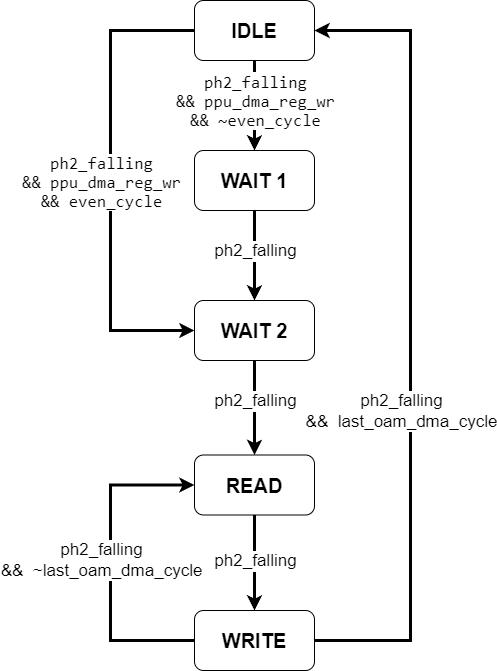
\includegraphics[width=120mm, keepaspectratio]{figures/sprite-dma-FSM}
\caption{OAM DMA működési állapotgépe} 
\label{fig:sprite-dma-FSM}
\end{figure}

Ezt a szinkronizációs problémát leszámítva, a hardver működése egyszerű. A CPU a DMA elérése során egy címet ad az eszköznek amely a CPU munka memória egy területére mutat általában \$0200. Majd innen az olvasási és írási állapotok váltakozásával 64 * 4 bájt memória mennyiséget olvas és ír (a teljes elsődleges OAM memóriát). Az írás a PPU \$2004-es OAM data regiszterére történik, ennek feldolgozását \aref{sec:fpga-sprite-rendering} fejezetben olvashatjuk.

A memória terület másolását követően az eszköz, vissza adja a CPU címbuszát és master adatbusz kimeneteit vissza állítom nullára, ezzel elengedve a CPU adatbuszt.

Egy DMA ciklus teljes szimulációját \aref{fig:Full-dma-working-in-simulation} képen láthatjuk, már itt is megfigyelhető, hogy a ready jel elvételét követően a DMA címbusza elkezd adni és ezek az értékek kerül ki a CPU összesített címbuszára. \Aref{fig:Working-dma-in-simulation} szimulációs képen pedig egy DMA ciklus kezdetét láthatjuk. Itt nyomon követhetjük a címbuszok pontos tartalmát. Tehát láthatjuk, hogy a DMA \$0200 címről kezd el olvasni (ezt a címet ciklusonként növeli) és a \$2004-es címre pedig ír. Az írás és olvasás váltakozását, pedig az RNW jel váltakozása mutatja. 

\begin{figure}[H]
	\centering
	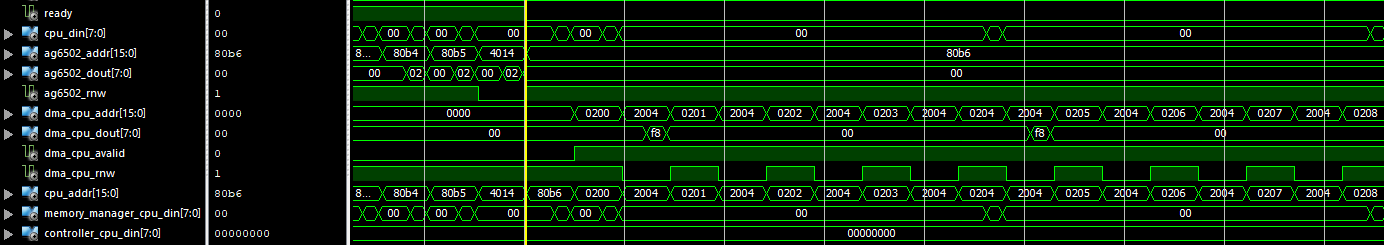
\includegraphics[width=150mm, keepaspectratio]{figures/Working-dma-in-simulation}
	\caption{A DMA ciklus kezdete szimulációban} 
	\label{fig:Working-dma-in-simulation}
\end{figure} 

\begin{figure}[H]
	\centering
	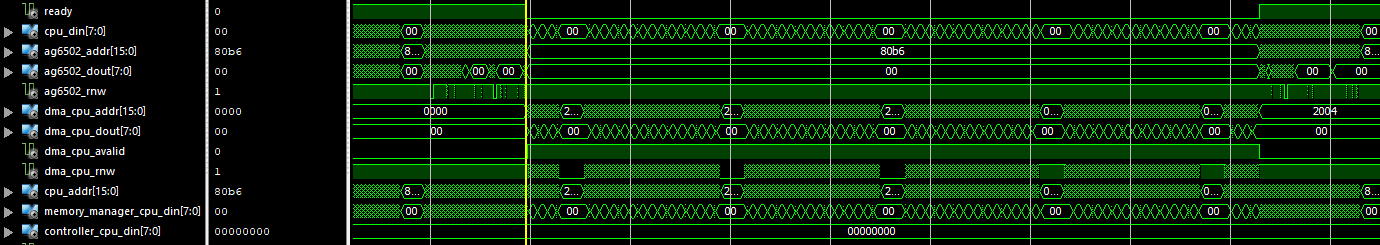
\includegraphics[width=150mm, keepaspectratio]{figures/Full-dma-working-in-simulation}
	\caption{Teljes DMA ciklus szimuláció} 
	\label{fig:Full-dma-working-in-simulation}
\end{figure} 

\section{6502 processzor működése az FPGA rendszerben}

A PPU és az eddig elkészített hardveres elemek tesztelhetősége véget, a projekt ezen fázisában inkább különböző Open Source processzorokat próbáltam a rendszerbe illeszteni. Itt nagy segítségemre volt az OpenCores nevű weboldal \cite{OpenCore}, amely különböző nyílt forráskódú processzorok és hardveres eszközök hardverleírását tartalmazta. Illetve a szintén nyílt forráskódú Mister NES projekt \cite{MisterNES}, amely rendelkezik egy VHDL nyelven íródott processzorral. Ezek rendszerbe illesztése viszont nagyon idő igényesnek érződött, ezért konzulensemhez fordultam segítségért. Szerencsére Raikovitch Tamás el tudott látni, egy általa készített és a karbantartott 6502-es processzor spartan-6-osra szintetizált és imlementált processzor binárisával binárisával a tesztelésekhez. Ez egy régebbi projektje során használt megbízható processzor implementációnak bizonyult, amelyet könnyen az eddig implementált rendszerembe tudtam illeszteni. \Aref{fig:working-cpu-simulation} szimulációs képen jól látható, hogy a rendszer helyesen képes beolvasni a Szuper Mario első utasítását, ez körülbelül a kép közepén a $cpu\_din$ csatornáján, 78-as (hexa) assembly kód. 

\begin{figure}[H]
	\centering
	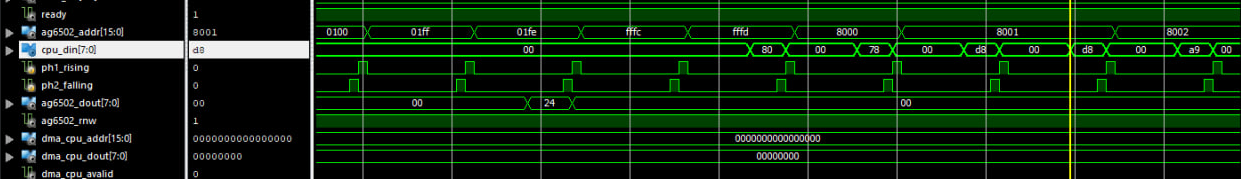
\includegraphics[width=150mm, keepaspectratio]{figures/working-cpu-simulation}
	\caption{A CPU szimulációja működés közben, Super Mario Bros. első assembly kódjának olvasása} 
	\label{fig:working-cpu-simulation}
\end{figure} 

A CPU-nak köszönhetően, a tesztelések során biztos lehettem, hogy csak az általam létrehozott rendszerben van hiba és a processzor teljes mértékben jól működik. Ezt követően könnyebb lesz egy nyílt forráskódú 6502 illesztése a NES-embe mivel biztos lehetek, hogy az általam készített hardver helyesen, az eredeti NES-nek megfelelően működik. 

\section{NES kontrollerek kezelése}

Az eredeti NES kontrollerek működését \aref{sec:NES-controller} fejezet során már ismertettem. Az FPGA implementáció során a modul feladata a kontrollerek párhuzamos-soros léptető regiszterei felé a vezérlő jelek küldése, tehát az olvasási szándék jelzése $controller\_out\_latch$, illetve a bitek olvasását követő órajel küldése $controller_1-_2\_out\_clk$. A kontrollerekből érkező adatok mintavételezésére, egy felfutó él érzékelést készítettem a CPU \$4016-as (kontroller 1) és \$4017-as (kontroller 2) regiszterének olvasására annak érdekében, hogy mindig stabil adatokat olvassunk (az olvasás egyszer történjen meg). Az élérzékelést egy-egy kétbites léptetőregiszterrel implementáltam, amelyekbe egyes értéket léptetek a jelek érkezésekor.   

A kontrollerekből érkező egybites adatokat, a CPU egy bájt ként olvassa ki (az adat a 0. helyi értékű biten szerepel). A CPU adatbusz kezelése során itt is figyeltem az interfész helyes implementációjára, tehát a $ph_2\_falling$ jel hatására nullás értékre állítom a CPU adat kimeneteket. A modulban mind a két kontroller írását és olvasását elhelyeztem.
